 \documentclass{article}

\usepackage[francais]{babel}
\def\printlandscape{\special{landscape}}    % Works with dvips.
%\usepackage{pstricks,pst-node,pst-tree}
%\usepackage{amssymb}
\usepackage{amsmath}
\usepackage[utf8]{inputenc}
\usepackage[T1]{fontenc} 
\usepackage{fancybox} % for shadow and Bitemize
\usepackage{alltt}
\usepackage{graphicx}
\usepackage{lmodern}
%\usepackage{epsfig}
%\usepackage{fullpage}
%\usepackage{fancyhdr}
%\usepackage{moreverb}
%\usepackage{xspace}
\usepackage[colorlinks,hyperindex,bookmarks,linkcolor=blue,citecolor=blue,urlcolor=blue]{hyperref}
%\usepackage{wrapfig}
\usepackage{epsf}
\usepackage{enumitem}
\usepackage{pifont}
\usepackage{hyperref}
\usepackage{authblk}

\begin{document}



\title{\textbf{Rapport de projet pluridisciplinaire :} \newline Diffusion non linéaire en sciences de la terre modélisation des glaciers}
\author{Tania Mendes, Mathieu Nguyen, Samson Petros, Yazid Bouhria, Elyas Assili, Maryam Aarab}
\maketitle
 
\vspace{50 mm}

\includegraphics[width=5cm, keepaspectratio=true, height=5cm]{Logo_Polytech_Sorbonne-2.png}\hfill
\includegraphics[width=5cm, keepaspectratio=true, height=5cm]{Logo_Sorbonne_Universite-2.png}



\author{} 


\newpage

\tableofcontents

%-----------------------------------------------------------
\newpage
\section{Introduction}\label{sec:intro}

L’écoulement d’un glacier dépend de plusieurs facteurs qui sont principalement l’accumulation de neige, la fonte de glace, la gravité et le niveau de la pente du lit rocheux.
Les écoulements sont considérés comme fluides, incompressibles, visqueux et non linéaires, d’où l’intérêt de les modéliser avec les relations de Stokes.
\newline
C'est un processus continu, mais il est très difficile de les résoudre analytiquement. Pour cela, les modélisateurs utilisent donc des méthodes numériques.
L’intérêt ici va être d’énoncer les relations générales de Stokes appliquées aux glaciers, d’énoncer le modèle Shallow Ice Approximation (SIA) afin d’en déterminer les avantages et les limites dans l’analyse de l’écoulement d’un glacier en fonction du temps.


Dans le cadre de ce projet, nous allons utilisé le langage Julia pour la résolution de systèmes d'équations différentielles par \textbf{différences finies} afin de pouvoir prédire l'écoulement glaciaire du Groenland.


%-----------------------------------------------------------
\section{Présentation des techniques de résolution}

\subsection{Pourquoi Julia ?}

Julia est un langage de programmation moderne et polyvalent, créé en 2009 par des chercheurs et ouvert au grand public en 2012. C'est un langage de haut niveau, dynamique et conçu pour des calculs scientifique. Sa syntaxe est similaire à Python, R ou encore Matlab.
 


\subsection{Les équations de Stokes}

Les équations de Stokes résultent des équations de Navier-Stokes: 
\begin{equation}
\Delta \mu v + \rho g = \rho \frac {\partial v}{\partial t}
\label{equ1}
\end{equation}
Le second membre correspond au terme d'inertie.  Ce terme peut être comparé aux effets visqueux par le nombre de Reynolds : 
\begin{equation}
\textit{Re} = \frac{\rho V L}{\mu}
\end{equation}
avec V une vitesse caractéristique et L une longueur caractéristique. 
Dans l'étude des glaciers, le nombre de Reynolds est faible ce qui nous permet négliger le second membre de ~\eqref{eq1} car ceux-ci s'écoulent lentement.
Cela nous permet d'obtenir l'équation suivante: 
\begin{equation}
\Delta \mu v + \rho g = 0
\end{equation}
Les équations de Stokes \cite{site1} ont comme principal objectif de décrire les mouvements des fluides. 
Pour procéder correctement, il faut connaître sa vitesse en tout point de l'espace : son champ de vitesse. Ainsi les équations de Stokes permettent de décrire le champ de vitesse d'un fluide. 
Dans un fluide nous considérons deux types de forces à savoir, les forces de volume (donc de poids) et les forces de surface correspondant aux frottements visqueux. 

Afin de pouvoir appliquer ces équations dans le cas des écoulements des glaciers, nous considérerons ces derniers comme des fluides incompressibles, visqueux et non linéaires. Il s'agit d'un système d'équations pouvant être appliqué à tout type de glacier.
\newpage
Ce système permet une très grande précision dans les résultats puisqu'il prend en compte toutes les contraintes au nombre de neuf, qu’elles soient longitudinales, transversales, verticales ou encore horizontales. 


L'équation de Navier-Stokes peut être assimilé à la deuxième loi de Newton appliquée aux fluides
\begin{equation}
\sum\vec{F}=m\vec{a}
\end{equation}
 , avec  $\vec{F}$ les forces s'exerçant sur le volume, $m$ sa masse et  $\vec{a}$  son accélération.
Étant donné que le nombre de Reynolds est petit, on peut négliger l'accélération ce qui nous mène à l'équation suivante:
\begin{equation}
\sum\vec{F}= 0
\end{equation}
Il faut alors déterminer les 3 termes pour un fluide en mouvement, à savoir dans notre cas, la glace. \newline
Les termes qui vont suivre sont explicités dans le cours "Introduction à la dynamique des fluides visqueux" de Thierry Menand.\cite{menand2020introduction}
\\\\
La masse d'un fluide se réécrit :
\begin{equation}
\Delta m = \rho \Delta V = \rho dxdydz
\end{equation}
Avec $\rho$ la masse volumique et $\Delta V =dxdydz $ le volume du fluide.
\\\\
Les 3 composantes de l'accélération d'un fluide dans un volume élémentaire s'écrit : 
%\begin{equation}
%%\begin{array}{l}
%%\frac{D v_{x}}{Dt} = \frac{\partial v_{x}}{\partial t} + (\vec{v}.\vec{\nabla})v_{x} = \frac{\partial v_{x}}{\partial t} + v_{x} \frac{\partial v_{x}}{\partial t} + v_{y} \frac{\partial v_{x}}{\partial t} + v_{z} \frac{\partial v_{x}}{\partial t}  \\
%%\frac{D v_{y}}{Dt} = \frac{\partial v_{y}}{\partial t} + (\vec{v}.\vec{\nabla})v_{y} = \frac{\partial v_{y}}{\partial t} + v_{x} \frac{\partial v_{y}}{\partial t} + v_{y} \frac{\partial v_{y}}{\partial t} + v_{z} \frac{\partial v_{y}}{\partial t} \\
%%\frac{D v_{z}}{Dt} = \frac{\partial v_{z}}{\partial t} + (\vec{v}.\vec{\nabla})v_{z} = \frac{\partial v_{y}}{\partial t} + v_{x} \frac{\partial v_{z}}{\partial t} + v_{y} \frac{\partial v_{z}}{\partial t} + v_{z} \frac{\partial v_{z}}{\partial t}
%%\end{array}
%\label{eq1}
%\end{equation}
\\\\
La somme des forces est la somme des forces $\vec{F}v$ qui agissent sur tout le volume et des forces $\vec{F}s$ qui agissent sur ces surfaces.
\\\\
Les forces de volume  $\vec{F}v$ induitent par la gravité, agissent sur toutes les particules du volume élémentaire et s'écrient :
\begin{equation}
\vec{F}v = 
\left(
\begin{array}{l}
F_{vx} \\
F_{vy} \\
F_{vz}
\end{array}
\right)
=
\left(
\begin{array}{l}
\Delta_{m} g_{x} \\
\Delta_{m} g_{y}  \\
\Delta_{m} g_{z} 
\end{array}
\right)
= \rho
\left(
\begin{array}{l}
g_{x} \\
g_{y}  \\
g_{z}
\end{array}
\right)
\Delta V
\end{equation}
 avec la masse $\Delta_{m} = \rho \Delta V$ et $g$ l'accélération de la pesanteur.
\\\\
Les forces de surface $\vec{F}s$ sont les forces induitent par la pression du fluide s'exerçant perpendiculairement aux surfaces et les forces induitent par les contraintes cisaillantes qui agissent parallèlement aux surfaces. Pour le cas d'un glacier nous prenons en compte que les contraintes normales à la surface : 
\begin{equation}
\sigma = 2 \mu \varepsilon - I_{d}P
\end{equation}
avec $\mu$ le coefficient de viscosité, $\varepsilon$ le taux de déformation, $I_{d}$ la matrice identité et $P$ la pression. $2\mu \varepsilon$ est la partie qui concerne la déformation et $I_{d}$ est la partie isotrope.\newline
Soit les 3 composantes des contraintes normales aux surfaces :
\begin{equation}
\left(
\begin{array}{l}
\sigma_{xx} = -P + 2 \mu \frac{\partial v_{x}}{\partial x} \\
\sigma_{yy} = -P + 2 \mu \frac{\partial v_{y}}{\partial y} \\
\sigma_{zz} = -P + 2 \mu \frac{\partial v_{z}}{\partial z}
\end{array}
\right)
\end{equation}
\\
Ainsi les forces de surface $\vec{F}s$ s'écrient : 
\begin{equation}
\vec{F}s = 
\left(
\begin{array}{l}
\sum F_{sx} = (-\frac{\partial P}{\partial x} + 2\mu \frac{\partial^2v_{x}}{\partial x^2})\Delta V  \\
\sum F_{sy} = (-\frac{\partial P}{\partial y} + 2\mu \frac{\partial^2v_{y}}{\partial y^2})\Delta V \\
\sum F_{sz} = (-\frac{\partial P}{\partial z} + 2\mu \frac{\partial^2v_{z}}{\partial z^2})\Delta V
\end{array}
\right)
\end{equation}
\\\\
Au final, en réécrivant la loi de Newton avec tous les termes, nous retrouvons :
\begin{equation}
\left(
\begin{array}{l}
\rho \frac{D v_{x}}{Dt} = \rho(\frac{\partial v_{x}}{\partial t} + v_{x} \frac{\partial v_{x}}{\partial t} + v_{y} \frac{\partial v_{x}}{\partial t} + v_{z} \frac{\partial v_{x}}{\partial t}) = \rho g_{x} - \frac{\partial P}{\partial x} + 2\mu \frac{\partial^2v_{x}}{\partial x^2}  \\
\rho \frac{D v_{y}}{Dt} = \rho(\frac{\partial v_{y}}{\partial t} + v_{x} \frac{\partial v_{y}}{\partial t} + v_{y} \frac{\partial v_{y}}{\partial t} + v_{z} \frac{\partial v_{y}}{\partial t}) =  \rho g_{y} - \frac{\partial P}{\partial y} + 2\mu \frac{\partial^2v_{y}}{\partial y^2} \\
\rho \frac{D v_{z}}{Dt} = \rho(\frac{\partial v_{y}}{\partial t} + v_{x} \frac{\partial v_{z}}{\partial t} + v_{y} \frac{\partial v_{z}}{\partial t} + v_{z} \frac{\partial v_{z}}{\partial t}) = \rho g_{z} - \frac{\partial P}{\partial z} + 2\mu \frac{\partial^2v_{z}}{\partial z^2}
\end{array}
\right)
\end{equation}
\\
Sous forme vectorielle l'expression se réécrit : 
\begin{equation}
\left\{
\begin{array}{l}
-div(2 \mu \varepsilon(\vec{v})) + \nabla p = \rho \vec{g} \\
div(\vec{v}) = 0 \qquad
\end{array}
\right.
\label{eq1}
\end{equation}
avec $\nabla = ( \frac{\partial}{\partial x} + \frac{\partial}{\partial y} + \frac{\partial}{\partial z})$, $\vec{v}$ la vitesse, $\vec{g}$ l'accélération de pesanteur, $\rho$ la masse volumique, $\mu$ le coefficient de viscosité et $\varepsilon$ le taux de déformation. $div(\vec{v}) = 0$ car il n'y a pas de variation de volume.
\\\\
Néanmoins, le Groenland est une calotte grande de milliers de kilomètres. Il faut alors un nombre considérable de points pour résoudre ces équations. De plus du fait de la complexité de celles-ci ainsi que des géométries de la calotte, cela est coûteux en temps de calcul. 


Il existe de nombreuses simplifications de  ces équations afin de minimiser le temps de calcul. Parmi elle, une des plus connue est l'approximation de la couche mince (Shallow Ice Approximation)appliquée pour la première fois sur la glace par Kolumban Hutter (1983). Ce modèle permet de réduire le problème de résolution 3D à un problème 2D. Il permet des calculs beaucoup plus simples. Ainsi, les calottes étant relativement minces, soit quelques kilomètres d'épaisseur, nous pouvons négliger les (variations verticales de la vitesse) les contraintes de cisaillement longitudinales et utiliser le modèle de l'approximation de la couche mince.

 \newpage
\subsection{Shallow ice approximation (SIA)}


Pour cette partie, nous nous sommes renseignées à travers le cours de Martina Schäfer \cite{schafer2007modelisation} et aussi grâce à un article publié dans le Cambridge University Press  \cite{seroussi_morlighem_rignot_khazendar_larour_mouginot_2013}.
\newline
Cependant, d'après une étude de ,des chercheurs assurent que la résolution du système des équations de Stokes est très couteuse en temps pour des applications réalistes (avec une complexité de \textbf{nlog(n)}. C'est pour cette raison qu'ils utilisent une simplification de ces équations basée sur le fait que sur de très grandes calottes, l'épaisseur est extrêmement faible par rapport à la dimension horizontale. Pour cela, nous allons utiliser le modèle SIA (Shallow Ice Approximation). Sa validité dépend du rapport d'aspect caractéristique $\zeta$ des objets glaciaires :
\begin{equation}
\zeta = \frac{e}{L}
\label{eq2} 
\end{equation}

Avec e l'épaisseur du glacier et L la largeur du glacier. Ce rapport est par exemple de $10^{-3}$ pour l'Antarctique et de $5.10^{-3}$ pour le Groenland. En effet, la validité de la SIA diminue lorsque le rapport d'aspect caractéristique $\zeta$ augmente. 

De plus, on néglige ici les interactions internes (aussi appelées bridge effect), ce qui nous permet de séparer les vitesses horizontales et verticales. $\mu$ est considéré isotrope et s'écrit :
\begin{equation}
\mu = \frac{B}{2\varepsilon(\vec{v})^\frac{n-1}{n}}
\label{eq2}      
\end{equation}
Où B est la solidité de la glace et n est le coefficient de la loi de Glen (on prendra n = 3)
\newline
La vitesse horizontale devient donc solution de :
\begin{equation}
-div(2 \mu \varepsilon(\vec{v}))  = \rho \vec{g}\frac{{\partial}S}{\partial x}
\label{eq3}
\end{equation}
L'évolution de la surface est déterminée en résolvant une équation hyperbolique, celle-ci est dictée par la conservation de masse. C'est cette équation que l'on retiendra car elle nous permettra d'étudier la hauteur de la glace au fur et à mesure du temps.
Cette équation s'écrit :
\begin{equation}
\frac{\partial H}{\partial t}=-\nabla H\vec{v} + Ms - Mb
\label{eq3}
\end{equation}
Avec H l'épaisseur de la glace, $\vec{v}$ la vitesse horizontale moyenne, \textit{Ms} la conservation de masse en surface et \textit{Mb} la fonte de la glace à la base.
Etant donné que $\vec{v}$ est la vitesse horizontale, c'est également une dérivée partielle selon x.
On peut donc écrire cette équation SIA comme la résolution d'une équation de diffusion non linéaire : 

\begin{equation}
\frac{\partial H}{\partial t}=D(H)\frac{{\partial}^{2}H}{\partial x^{2}} + M
\label{eq4}
\end{equation}

avec D le coefficient de diffusion, H l'épaisseur du glacier et M la conservation de masse.
\newpage
L'épaisseur H est donnée par l'équation suivante :
\begin{equation}
H(x) = S(x) + B(x)
\label{eq4}
\end{equation}
où B est la hauteur de l'encaissant rocheux et S la topographie de la glace. H est représentée sur la figure 1 : 
\\
\\
\begin{figure}[!htpb]
\centering
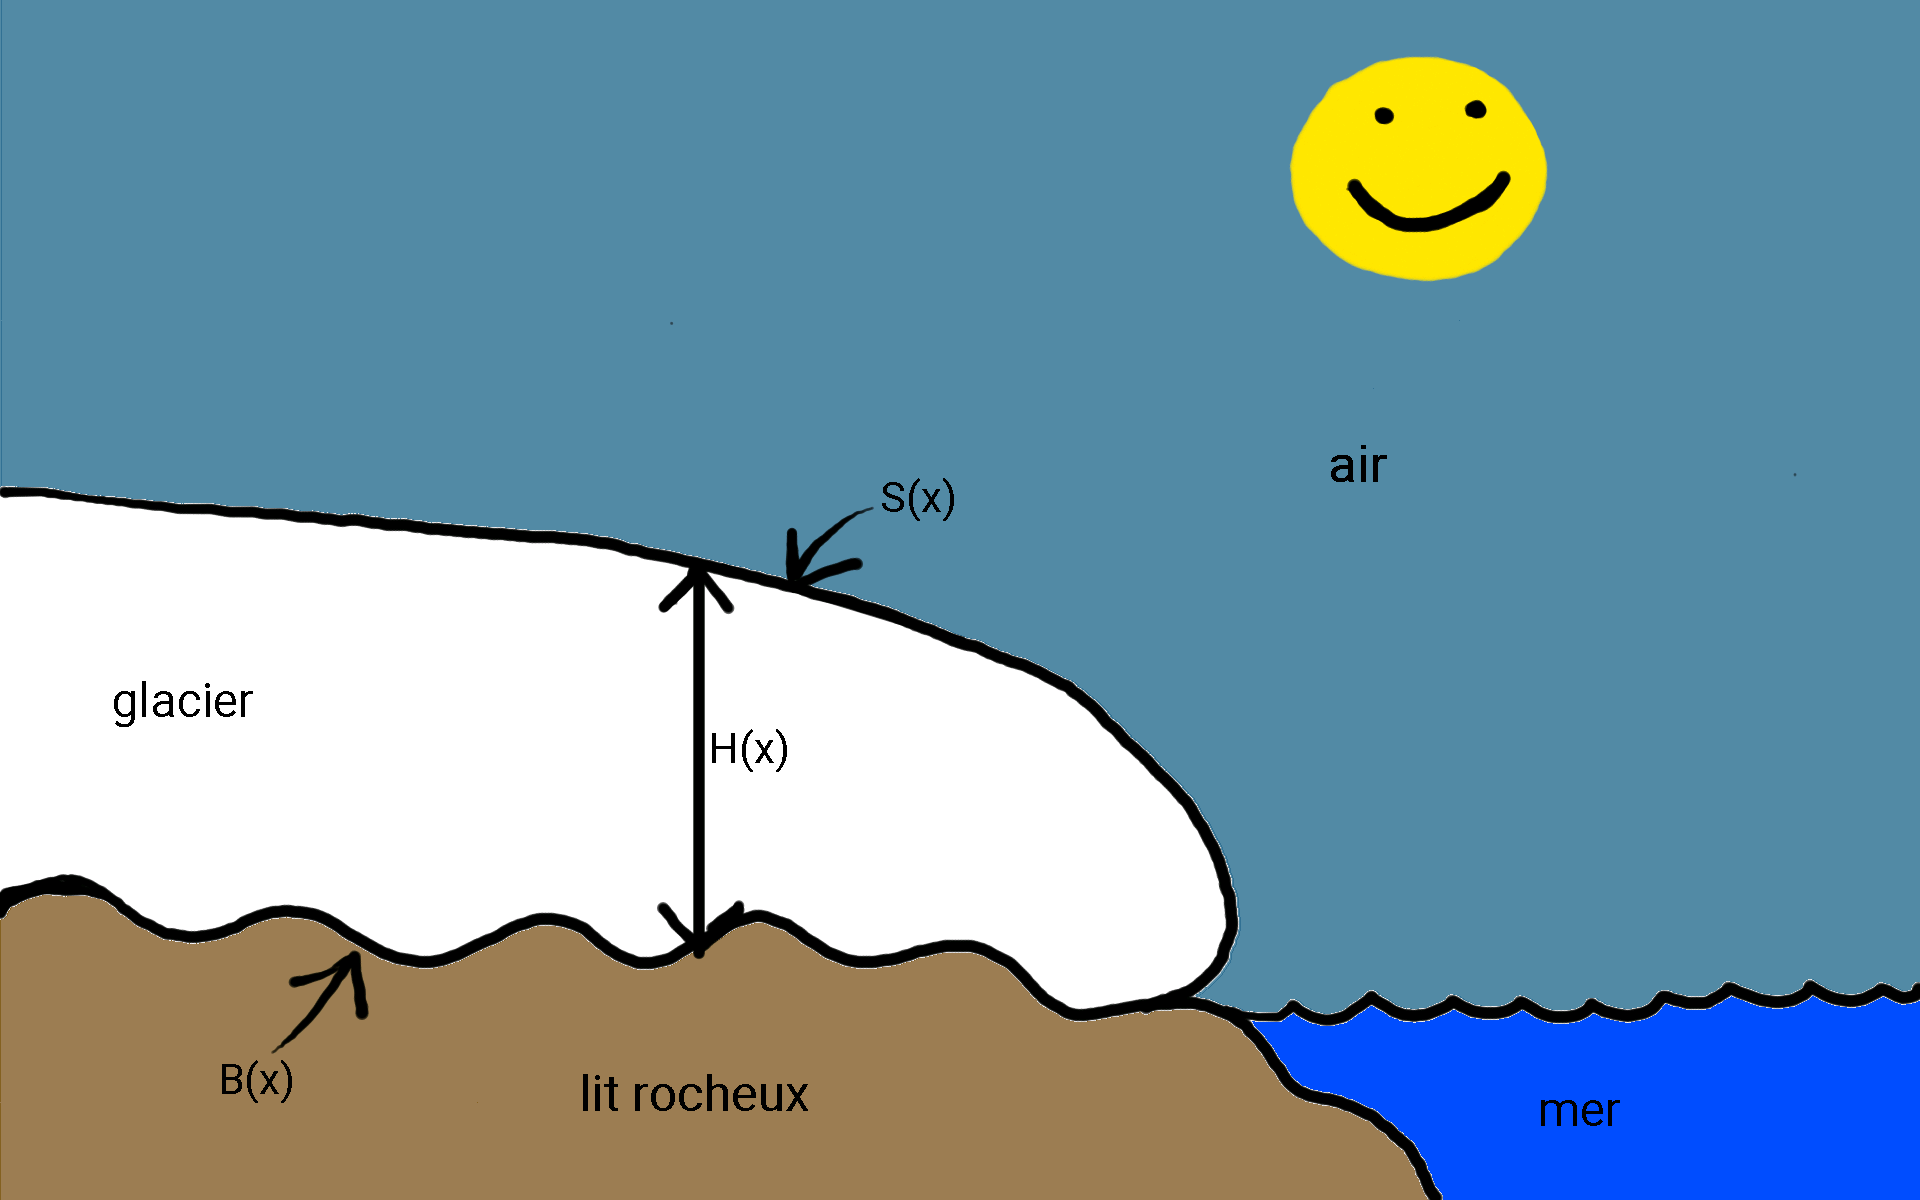
\includegraphics[width=10cm, keepaspectratio=true, height=10cm]{H.png}
\caption{Représentation de l'épaisseur de la glace H, la hauteur du lit rocheux B et la topologie de la glace S}
\label{fig01ch1}
\end{figure}
\newline
Les données topographiques, l'élévation du substratum rocheux et l'épaisseur de la glace proviennent du jeu de données BedMachine Greenland v3. 
\\

Il faut savoir que l'écoulement d'un glacier dépend de plusieurs facteurs : la neige, glace, pluie, fonte, perte de glace, gravité. La conservation de masse M se calcule de la manière suivante :
\begin{equation}
M = accumulation + ablation
\label{5}
\end{equation}

\newpage
Ainsi la conservation de masse permet d'équilibrer les 2 phénomènes à la surface en fonction de la ligne d'équilibre. L'altitude de la ligne d'équilibre (ELA) est où la zone d'accumulation, au sommet du glacier, est égale à la zone d'ablation, en bas du glacier. Nous pouvons la distinguer sur la figure 2 : 
\begin{figure}[!htpb]
\centering
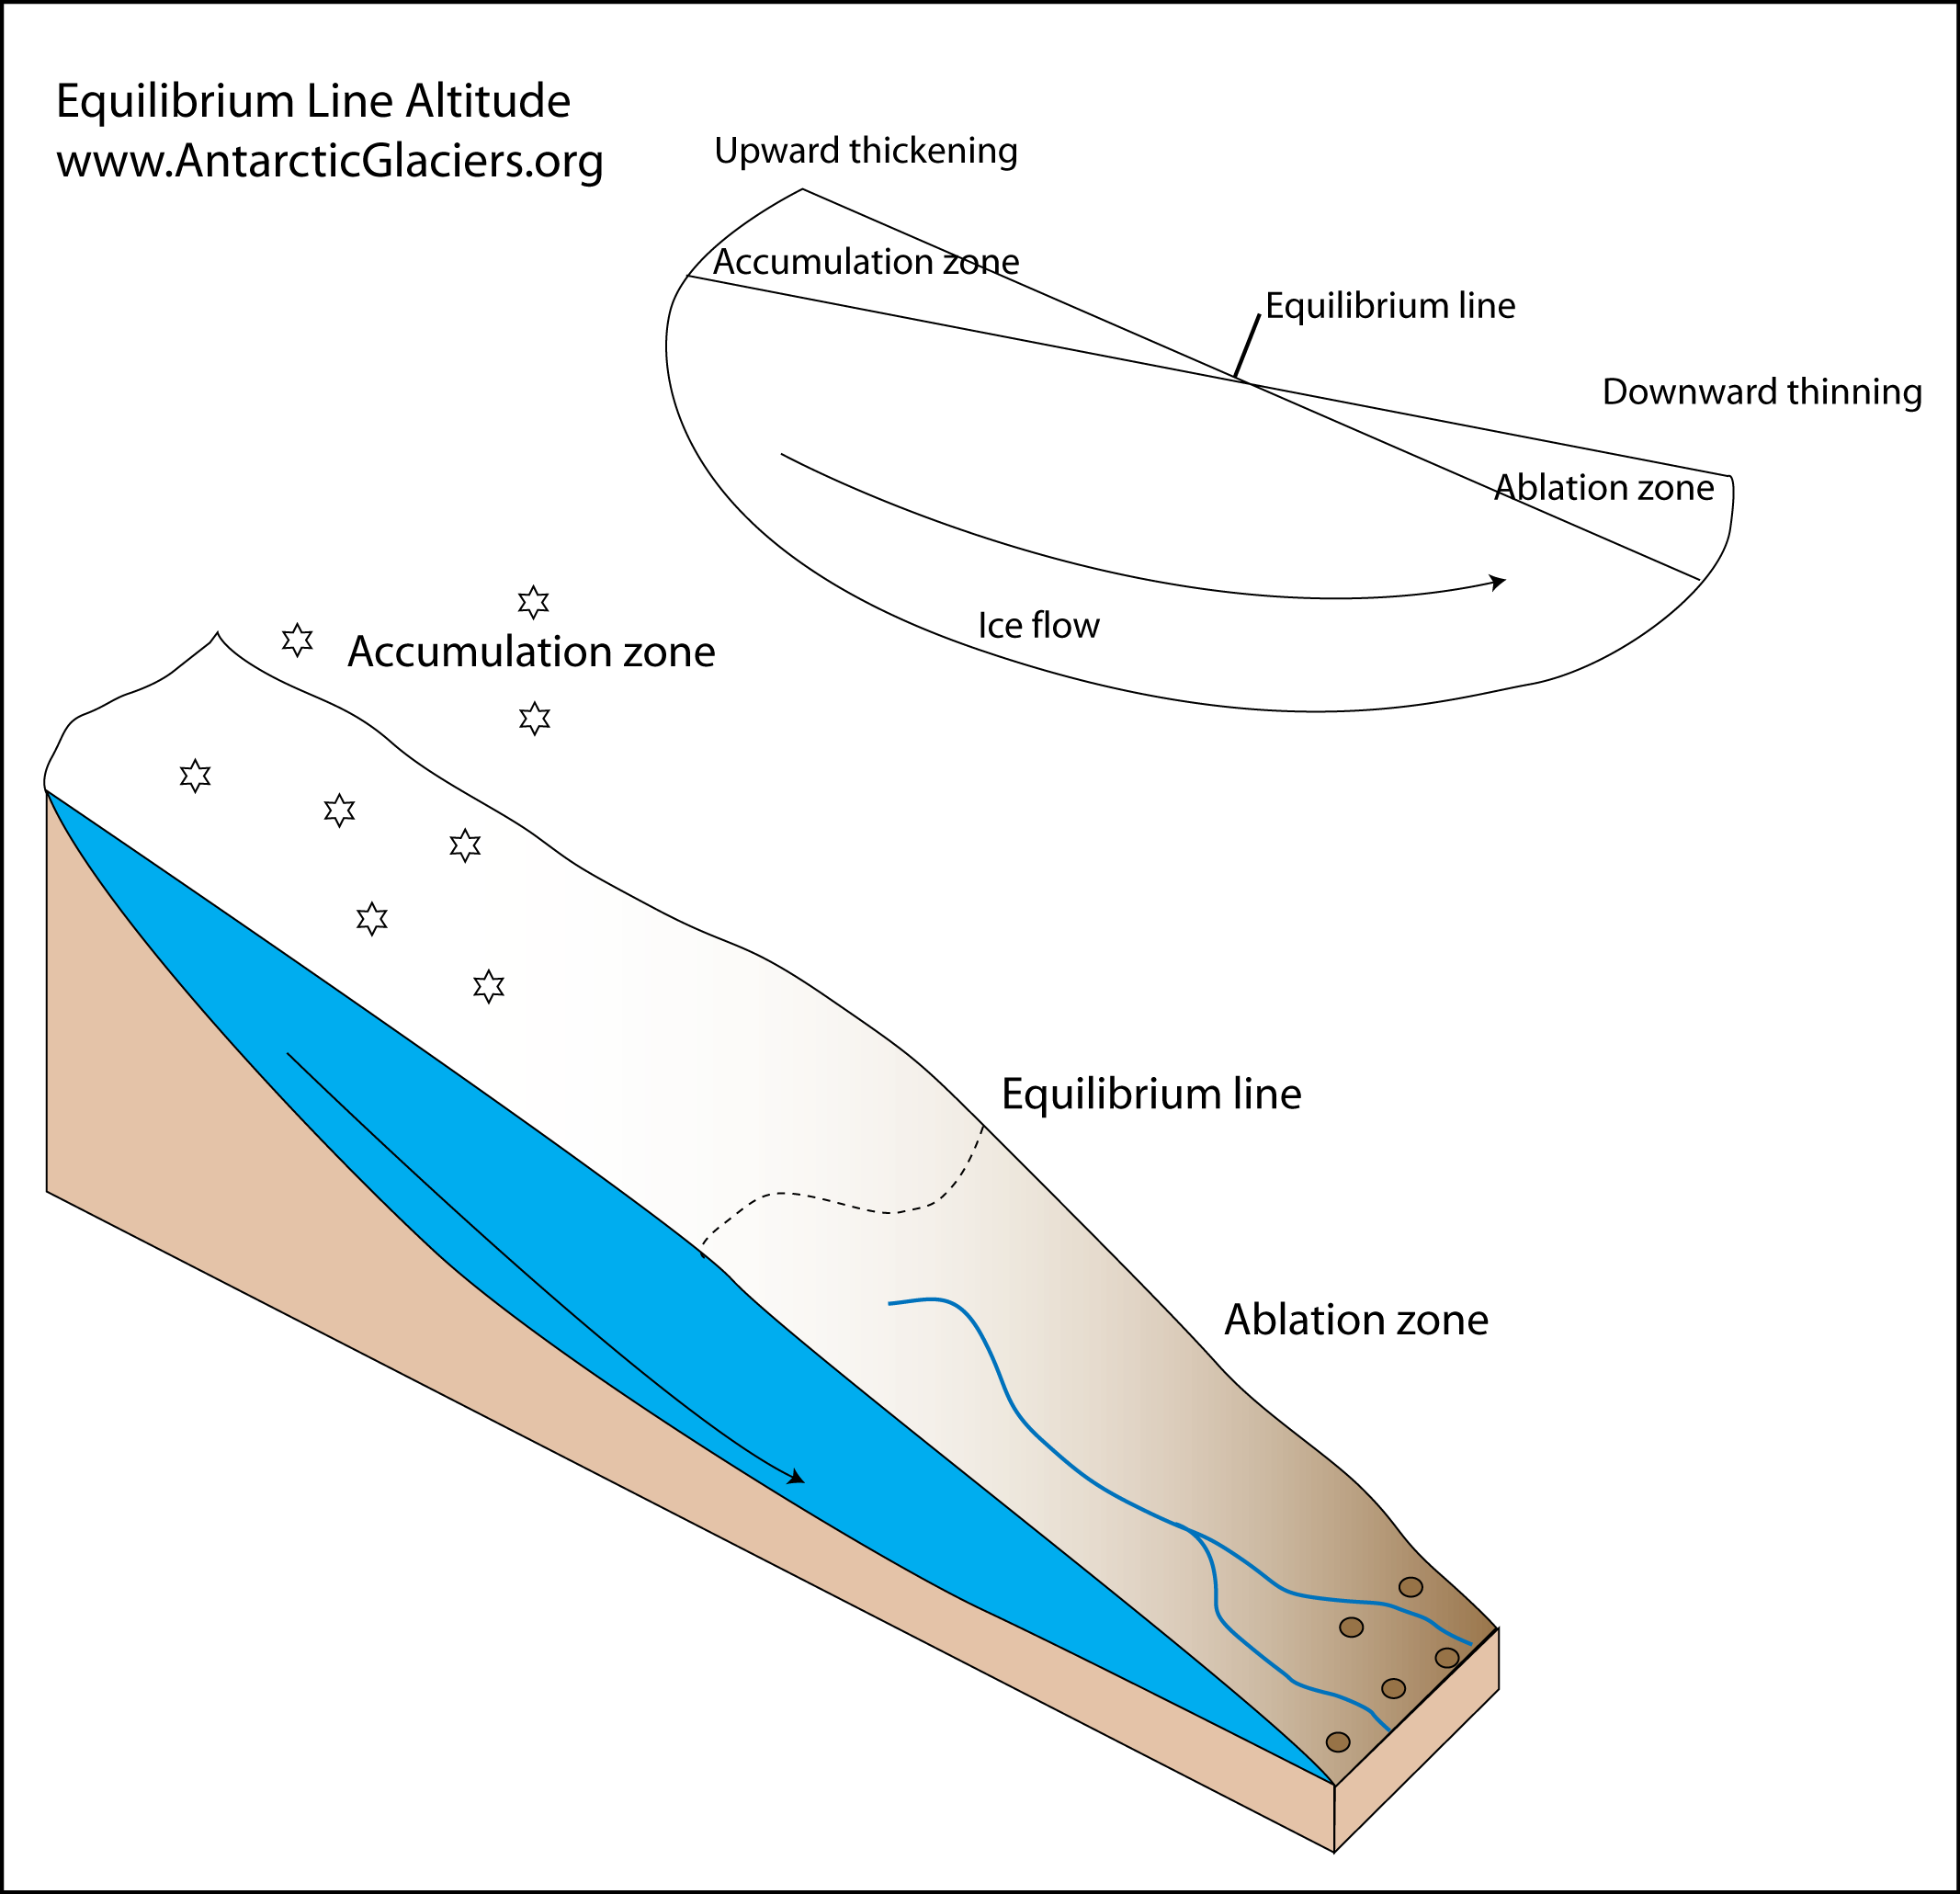
\includegraphics[width=10cm, keepaspectratio=true, height=10cm]{equilibrium_line_altitude1.png}
\caption{Représentation de la ligne d'équilibre sur un glacier, déterminée par la conservation de masse M, c'est-à-dire là où la zone d'abblation et la zone d'accumulation se rencontrent}

\end{figure}



Dans le code, la conservation de masse M est calculée à partir de \textit{gradb} (qui dépend de la lattitude) le gradient du bilan massique, \textit{zELA} l'altitude de la ligne d'équilibre (ELA) et \textit{bmax} l'accumulation maximale.
\newpage
\section{Simulations numériques}

Nous avons commencé par étudier un dossier GITHUB public \cite{site2} qui modélisait la fonte de glacier.
\newline

 Il était composé de trois codes qui résolvent l'équation de diffusion linéaire avec diférentes méthodes en 1D. Tout d'abord un premier code explicite. Un deuxième code qui rajoute une solution itérative ainsi qu'une tolérance de fin, forçant le programme à s'arrêter uniquement lorsque cette tolérance est atteinte. Enfin, un troisième code introduit un "damp" itératif qui permet au programme de converger plus rapidement.
\newline
Ces trois codes sont considérés linéaires, car le coefficient de diffusion D était une constante.
\newline
Un quatrième code considérait le problème de l'écoulement des glaciers à l'aide du SIA en 2D. Il inclut des itérations non linéaire, c'est-à-dire que ce coefficient D variait à chaque point et à chaque itération du problème, ainsi que les conditions initiales provenants des données. Notre but était donc de mieux comprendre le fonctionnement du code en 2D, puis en écrivant à notre tour un code 1D non linéaire qui résout le problème de SIA.
\newline
En s'inspirant de ces codes, nous avons créé un code dont la boucle s'effectue de la manière suivante :
\newline
\begin{verbatim}
while err>tolnl && iter<itMax # On sort lorsque l'erreur est en 
dessous de la tolérance 	(ou trop d'itérations)
        Err         .= H                                               
        M           .= min.(grad_b.*(S .- z_ELA), b_max)            
        dSdx        .= diff(S)/dx 
        D           .= a*av(H).^(npow+2) .*dSdx.^(npow-1)              
        qH          .= .-av(D).*diff(S[1:end-1])/dx                     
        ResH        .= .-(diff(qH)/dx .+ inn(M[1:end-1])) 
        dtau        .= dtausc*min.(10.0, cfl./(epsi .+ av(D[2:end])))
        dHdt        .= ResH + damp.*dHdt                                
        H[2:end-2]  .= max.(0.0,H[2:end-2] .+ dtau.*dHdt)               
        H[Mask.==0] .= 0.0
        S           .= B .+ H                                       
\end{verbatim}
\newpage
Nous avons recréé l'équation~\eqref{eq4} en calculant les dérivées partielles selon ${x}$ avec la méthode des différences finies. Cela consiste à calculer la différence entre deux valeurs consécutives. L'idée était de reprendre un code similaire au code non linéaire 2D et de ne conserver qu'une seule dimension, c'est-à-dire toutes les variables dépendantes de x. Les composantes dépendantes de y n'ont donc pas été prise en compte.
\newline
Nous avons introduit plusieurs tableaux : le coefficient de diffusion D, le flux qH, le résidu de l'équation ResH ainsi que les surfaces B, H et S, dont la taille varie en fonction des calculs qu'on leur applique. Par exemple, les méthodes des différences finies sur un tableau de taille nx renvoie un autre tableau de taille nx-1 (car on applique nx-1 opérations sur nx valeurs).
\newline
Ce code remet à jour toutes les valeurs jusqu'à ce que l'erreur déterminée descende en dessous d'une tolérance prédéfinie. On introduit également un pas d'itération maximal pour éviter que le programme ne s'arrête jamais.
\newline
A chaque tour de boucle, nous réinitialisons le coefficient D, la conservation de masse M et la [dérivée itérative] dtau. Puis nous calculons les dérivées partielles dSdx, qH et ResH en effectuant les différences finies. Toutes ces valeurs nous permettent de mettre à jour la [] dHdt ainsi que l'épaisseur de la glace H et enfin la surface S. Nous appliquons également un masque afin de ne pas atteindre le niveau de la mer et nous gardons en mémoire l'épaisseur H afin d'en déterminer l'erreur.
\newline
Au bout de cinquante itérations, nous actualisons la valeur de la variable err avec le code suivant :
\begin{verbatim}
if mod(iter, nout)==0 
            Err .= Err .- H
            err = norm(Err)/length(Err) 
end
\end{verbatim}
La boucle s'arrête lorsque l'erreur est plus petite que la tolérance imposée.

\section{Résultats}


Pour s'assurer que le code compilait, nous avons simplifié certaines variables du problème. La conservation de masse était constante et les surfaces H, B et S  étaient modélisées par des fonctions mathématiques. Une fois cela fait, nous avons extrait des valeurs d'un autre fichier contenant toutes les valeurs du Groenland [retrouver la référence].
\begin{figure}[!htpb]
\centering
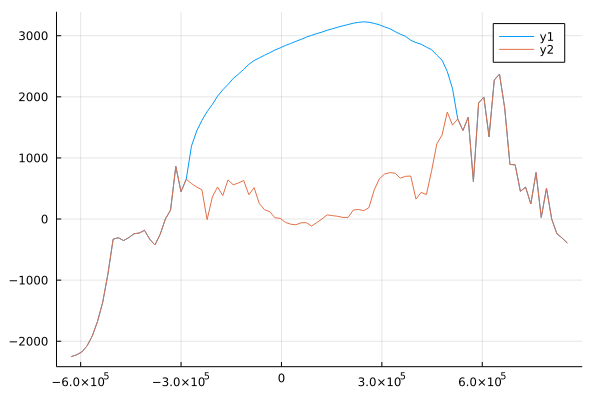
\includegraphics[width=10cm, keepaspectratio=true, height=10cm]{Groenland.png}
\caption{Topologie du Groenland d'après les données récupérées. La courbe y2 représente la hauteur du lit rocheux B et y1 la topologie de la glace S. }

\end{figure}
\newpage
Nous avons ensuite réajusté l'ablation M ainsi que les coefficients itératifs damp afin d'avoir une vitesse de convergence adaptée au problème.
Nous affichons donc le résultat obtenu à l'aide d'un plot.
\begin{figure}[!htpb]
\centering
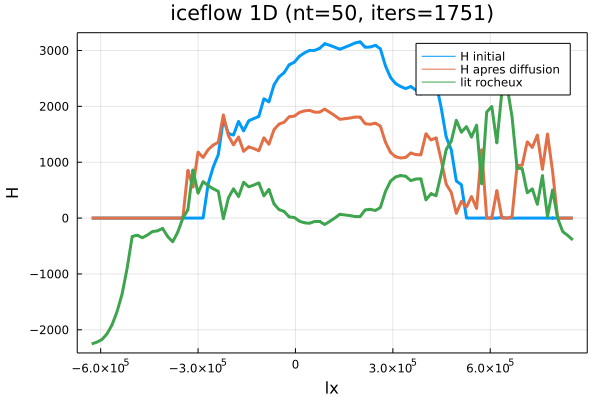
\includegraphics[width=10cm, keepaspectratio=true, height=10cm]{Iceflow1D.png}
\caption{Evolution du niveau de glace en fonction du temps. La courbe bleu représente la hauteur H au début, la courbe orange donne la hauteur H une fois la simulation terminée et la courbe verte montre le lit rocheux B.}

\end{figure}
\newpage
Il nous faut à présent déterminer la ligne où les variations verticales soient les plus faibles, afin d'avoir le modèle le plus proche possible de la réalité adapté a notre code.
\newline
Pour cela, nous avons cherché dans les données que nous avions sur le Groenland la ligne "horizontale" qui nous permettait d'avoir des résultats suffisamement justes pour pouvoir appliquer notre code. Plus précisemment, il fallait que la ligne choisie soit une ligne qui permette de négliger les vitesses verticales.
Pour choisir judicieusement cette ligne, nous avons comparé les différentes données de vitesses verticales \textit{Vy} que nous avions à notre disposition en faisant une somme entre deux lignes consécutives, voici le code qui nous a permis de trouver  la ligne correspondante: 
\begin{verbatim}
V = sqrt.(Vy.^2)
s=zeros(95)
for i = 1:95
    t=V[i,:]
    s[i]=sum(t)
end

for i = 2:94
    s1[i-1] = s[i-1] + s[i+1]
end
display(plot(1:95, s))
display(plot(1:94, s1))
\end{verbatim}
A l'aide de ce programme, nous pouvons obtenir une courbe donnant les vitesses verticales sur chaque ligne :
\begin{figure}[!htpb]
\centering
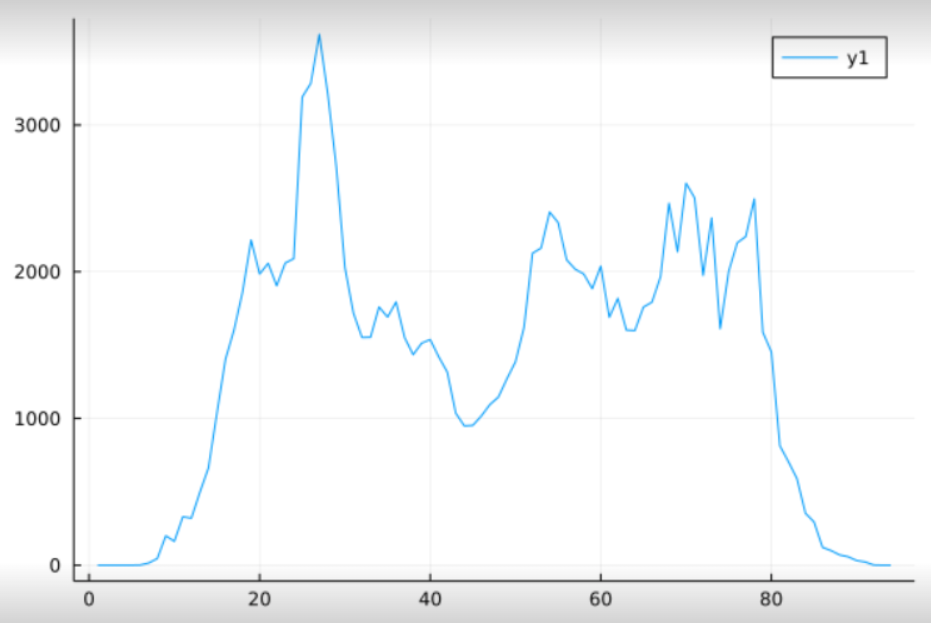
\includegraphics[width=10cm, keepaspectratio=true, height=10cm]{Vitesses.png}
\caption{Graphe représentant la somme des vitesses selon l'axe Y pour chaque ligne. On ne considère pas les bordures du Groenland car on veut prendre la ligne qui correspond au rapport entre la vitesse horizontale et verticale la plus élevée, ceci est situé au centre du Groenland }
\end{figure}
\newline
 En regardant au centre, nous observons que les vitesses verticales sont les plus faibles vers la ligne 43. Nous avons alors choisi cette ligne pour que notre modèle soit le plus cohérent avec notre modèle 2D. 
\newline
En exécutant le code avec cette ligne, nous avons alors le résultat suivant: 
\begin{figure}[!htpb]
\centering
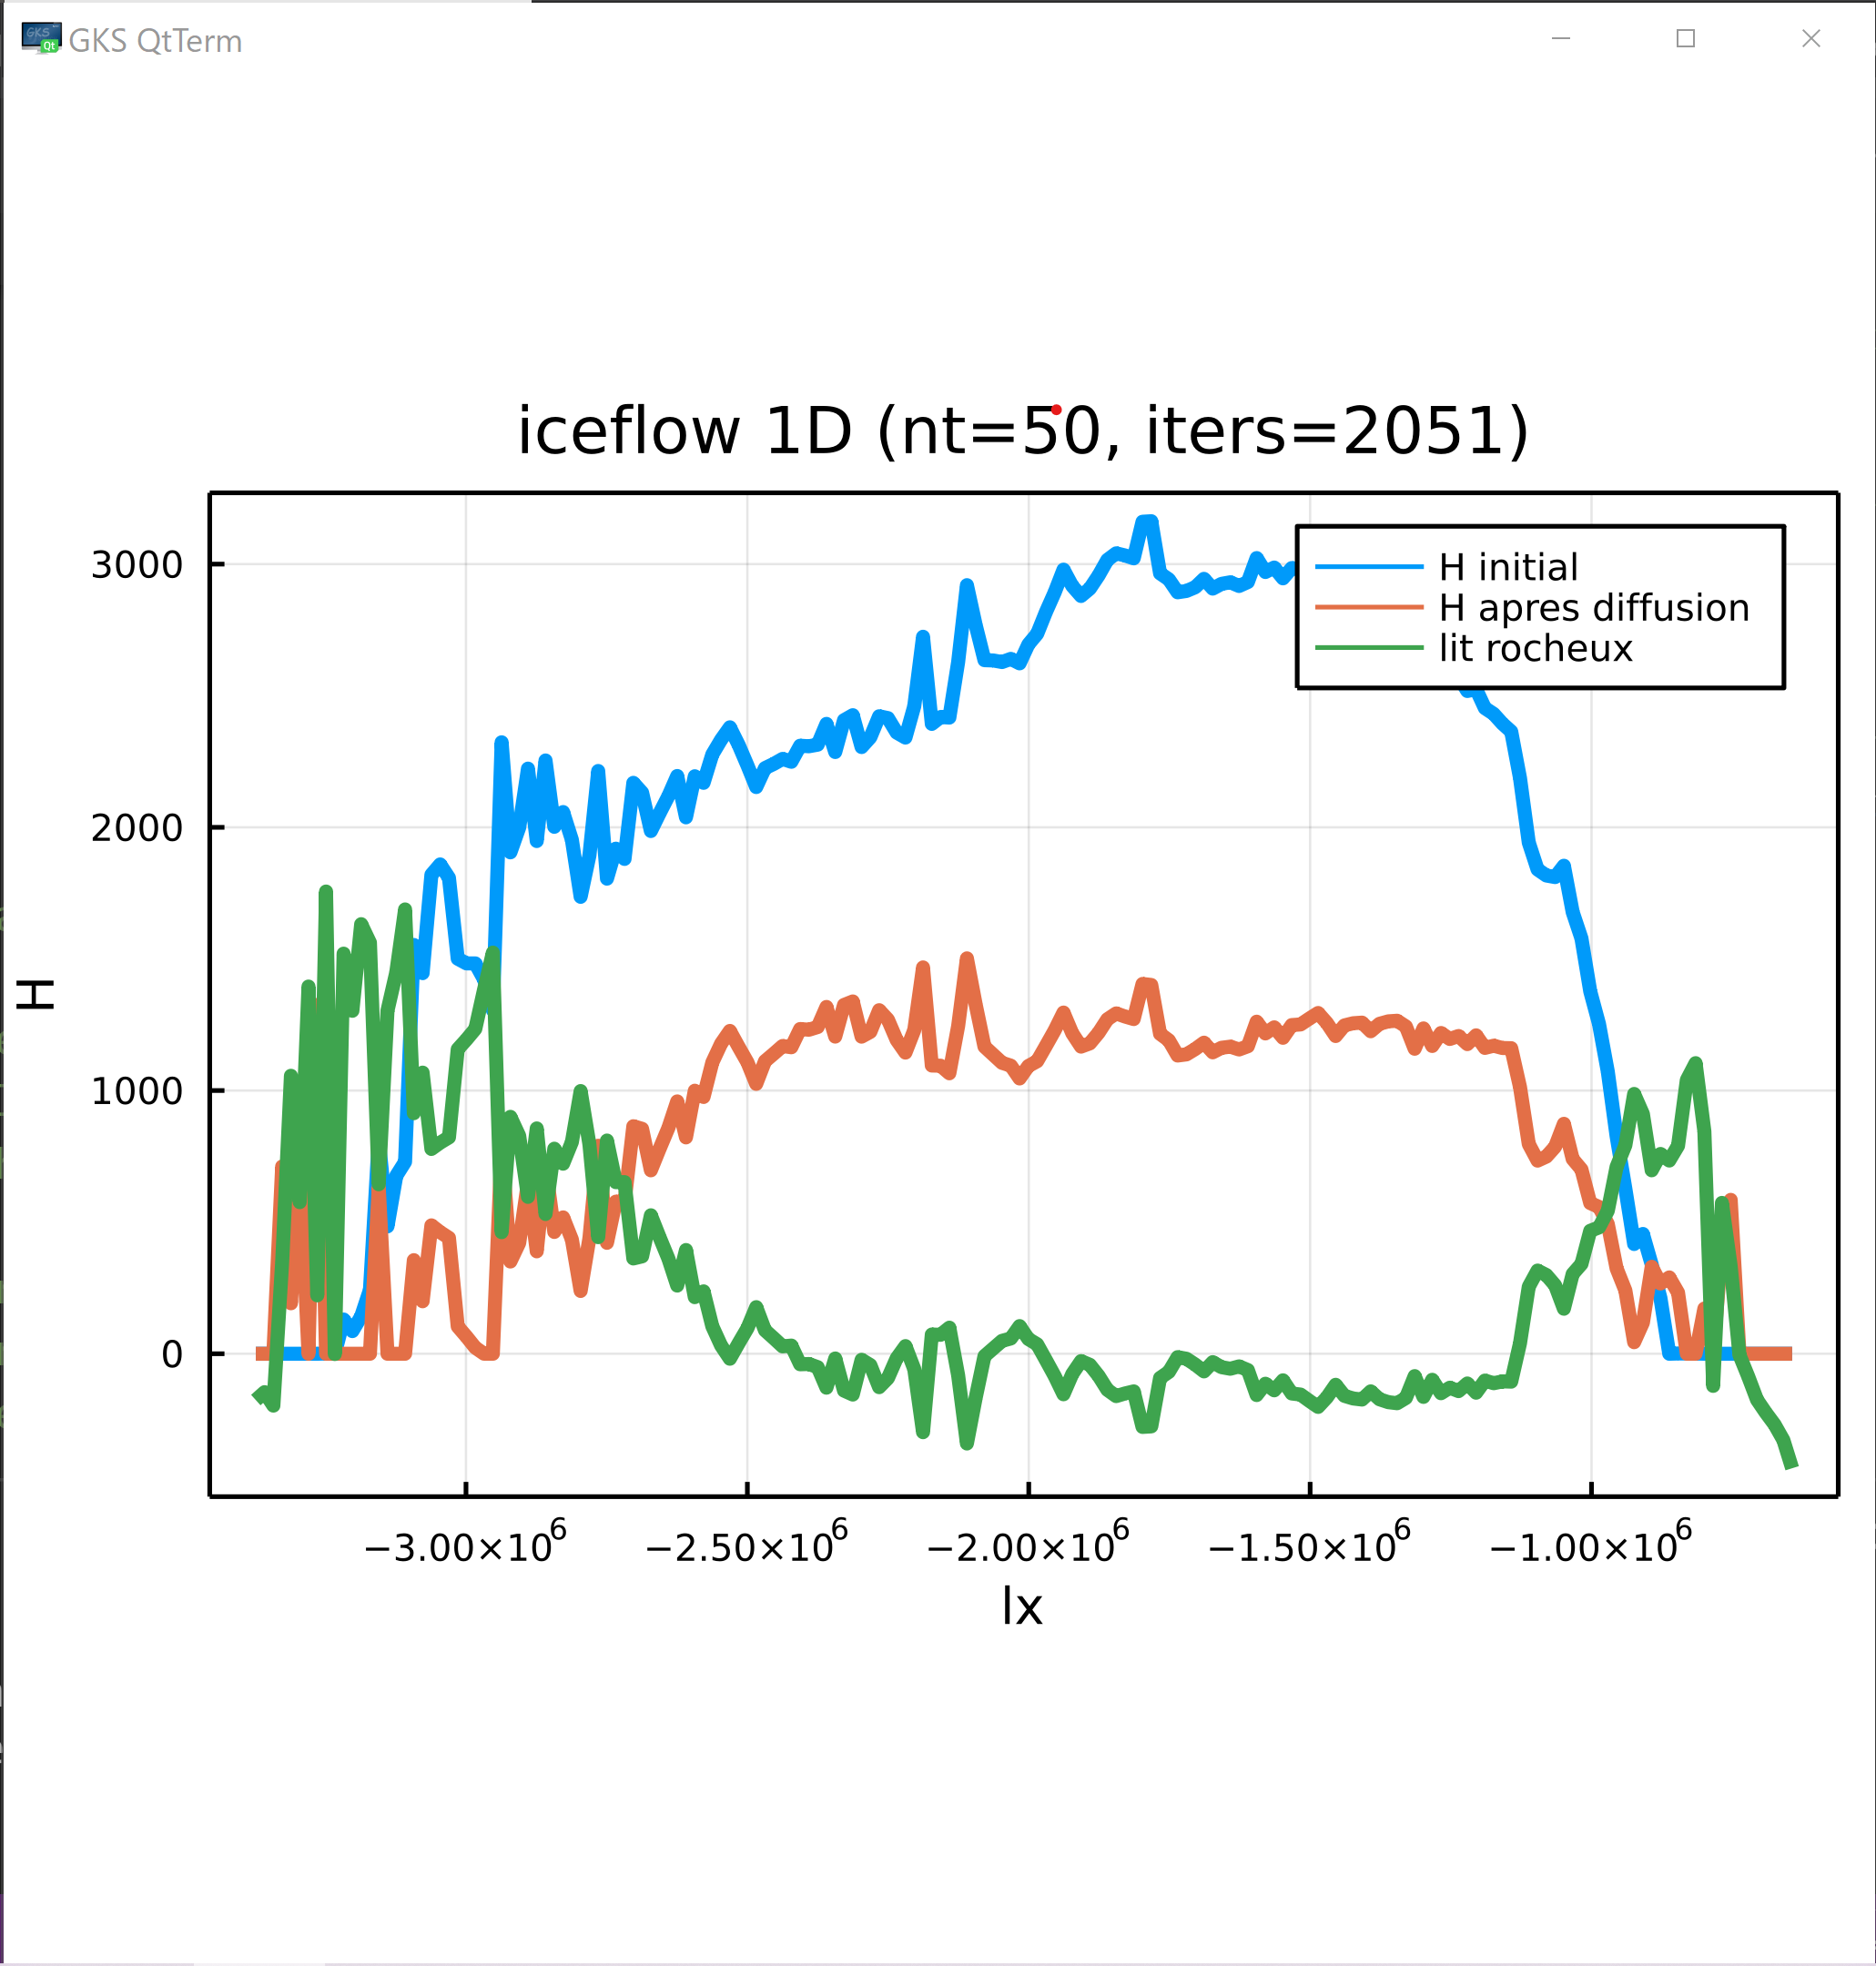
\includegraphics[width=10cm, keepaspectratio=true, height=10cm]{ligne43.png}
\caption{Topologie du Groenland en appliquant la ligne 43. La courbe bleue  représente la hauteur H au début, la courbe orange donne la hauteur H une fois la simulation appliquée pour la ligne 43 et la courbe verte montre le lit rocheux B. }
\end{figure}
\newpage
En observant notre schéma, nous pouvons à présent simuler l'évolution de la glace du Groenland et créer notre propre scénario. En conservant nos valeurs, nous pouvons observer une fonte de glace allant de 0 à 1500m de variation. Avec un simple calcul de moyenne, nous obtenons une variation moyenne de 1091m. Notre hauteur de base moyenne étant de 1907, cela nous donne une variation de 57\% de la hauteur. A chaque itération, nous réattribuons des valeurs à tous les tableaux en fonction de a, qui est la viscosité de la glace \textbf{calculée avec un pas de temps annuel}. Nous en déduisons qu'une itération correspond à une année et donc que ce scénario sera atteinte au bout de 2051 ans. 
\newline
Nous avons trouvé un article \cite{charbit2008amount} spéculant la fonte de glace au Groenland en fonction de la hausse de CO2, car celui-ci est directement relié avec la hausse de température. Il effectue plusieurs simulations, en fonction de la variation de température considérée (variant entre 1.1°C et 6.4°C) : 
\begin{figure}[!htpb]
\centering
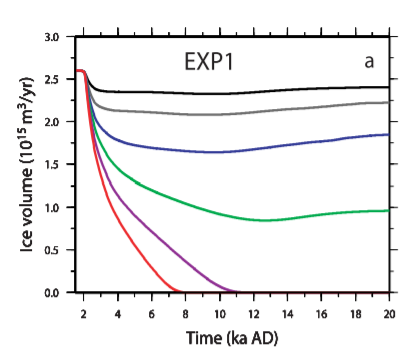
\includegraphics[width=10cm, keepaspectratio=true, height=10cm]{Variation.png}
\caption{Schéma indiquant le volume de glace du Groenload à partir de l'an 2000. Grâce à cette simulation, nous pouvons en déduire que le Groenload perdrait entre 10\% et 63\% de son volume, ce que l'on retrouve bien avec notre simulation (Notre simulation est proche de la courbe verte de ce schéma) }
\end{figure}
\newpage
% Faire différents scénarios en fonction de la fonte des glacier (3 ?)

%-----------------------------------------------------------
\bibliography{bibliographie.bib}
\bibliographystyle{unsrt}
\end{document}

%%% Local Variables:
%%% mode: latex
%%% TeX-master: t
%%% coding: utf-8
%%% End:
